% !TEX encoding = UTF-8 Unicode
%!TEX root = ../Main/thesis.tex
% !TEX spellcheck = en-US
%%=========================================
\documentclass[../Main/thesis.tex]{subfiles}
\begin{document}
\chapter[One class SVM coupled with wavelet transform for bearing health monitoring]{One class SVM coupled with wavelet transform for bearing health monitoring}
\label{sec:waveletandsvm}
In this chapter we introduce yet a another method for bearing fault detection. In Chapter \ref{sec:chapter2} We showed how the fast Fourier transform is applied to bearing fault diagnosis. Although popular in the industry for bearing fault analysis and detection, the fast Fourier transform method is not without limitations. As in any scientific methods, the limitations are grounded in the mathematical assumptions upon which the method is derived. As pointed previously, two such assumption are linearity, and stationarity. Furthermore, for bearing fault analysis, the fast Fourier method relies on the rotational speed of the motor on which the bearings are mounted. In addition, the forcing frequencies are derived from the physical properties of the bearing. Thus, the fast Fourier transform method for bearing fault detection can be seen as a physics base data driven method.
\justify
In this chapter, a purely data driven method is presented. It consists of applying wavelet transform for feature generation, a robust statistical estimator to quantify a bearing health, and a support vector machine (SVM) for anomaly detection. Before giving a detail account of the method, let clarify some semantics and outline the benefits of this method. A feature in the context of this chapter, is a component of a signal. As pointed out earlier, a signal can have multiple components, which can be extracted for example by applying Fourier series or Fourier transform. In this case a feature or component of the original signal is a trigonometric function. A support vector machine (SVM) is an algorithm for pattern identification that uses margins to separate data into different groups [vapnik1995].
\justify
The method presented in this chapter solely relies on the data to detect any fault. it does not require bearing physical properties, and can be applies to any nonlinear and non-stationary data generated process. In the rest of this chapter we will refer to a generic bearing fault as an anomaly. As defined in [chandola2009], \say{Anomalies are patterns in data that do not conform to a well defined notion of normal behavior}. In section \ref{sec:svm} a detailed account of support vector machine algorithm is lade out, followed by wavelet transform in section \ref{sec:wavelet}. Finally, section \ref{sec:sectionresult} presents a one class SVM coupled with wavelet transform for bearing anomaly detection.

%%%%%%%%%%%%%%%%%%%%%%%%%%%%%%%%%%%%%%%%%%%%%%%%%%%%%%%%%%%%%%%%%%%%%%%%%%%%%%%%%%%%%%%%%%%%%%%%%%%
%%%%%%%%%%%%%%%%%%%%%%%%%%%%%%%%%%%%%%%%%%%%%%%%%%%%%%%%%%%%%%%%%%%%%%%%%%%%%%%%%%%%%%%%%%%%%%%%%%%
\section{Support vector machine (SVM)}
\label{sec:svm}
The Support vector machine was originally presented by [vopnikk1995] as a two-groups, classification algorithm. It solves the problem of classifying an input vector into two groups. In the context of bearing fault detection: healthy versus unhealthy bearing would be the two groups. It was originally introduced as support-vector Networks, but is now popularly refer to as support vector machine. The bulk of the SVM rests on the following idea: Use a nonlinear kernel to map the input data into a high dimensional feature space, where a linear decision function is used to classify data into two groups.
\justify
A non linear kernel is just a nonlinear function and a decision function also called a discriminator function is a curve that separates the two groups. The classification is based on optimizing a margin separating the two groups. 
\begin{figure}[H] %  figure placement: here, top, bottom, or page
   \centering
   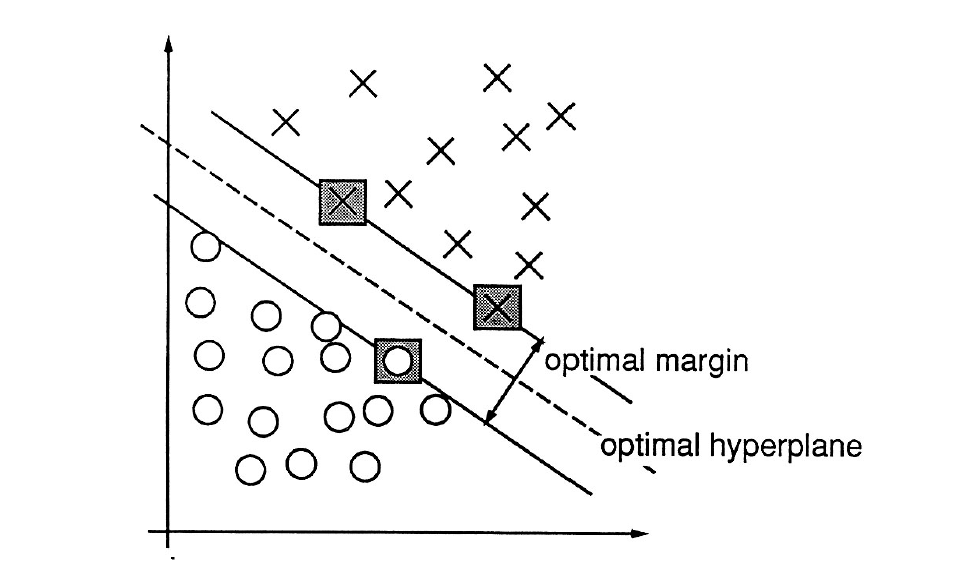
\includegraphics[width=5in]{../fig/svm2d.png} 
   \caption{Illustration of two classes classification from [vapnik1995]}
   \label{fig:svm2d}
\end{figure}
\justify
Figure \ref{fig:svm2d} shows a two groups classification problem. Two set of points marked by circle and cross are separated by the optimum curve or hyperplane (here the solid dash line). The margin is the distance or gap between solid dark lines. Here the two classes are linearly separable, meaning that a linear function can be used to separate the two classes. Support vectors are points that lies on the margins (points in grey square lying on the dark lines) and defines the margin of largest separation between the two classes [vapnik1995].
\justify
The formulation of the SVM problem goes like this: Let $\bm{X} \in \mathbb{R}^{d}$  be an input vector, $\bm{W}\in \mathbb{R}^{d}$ a vector of parameters and $b\in \mathbb{R}$, where $d$ is an integer. Let $y_{i}\in \{-1,1\}$. We can then classify a vector $\bm{X}_{i}, i = 1,\cdots,n$ such that
\begin{equation}\label{eq:svmformulation}
\begin{split}
\bm{W}^{T}\bm{X}_{i} + b &< 0, \quad \Rightarrow y_{i} = -1\\
\bm{W}^{T}\bm{X}_{i} + b &> 0, \quad \Rightarrow y_{i} = 1,
\end{split}
\end{equation}
where the equation of the separating hyperplane is then given by 
\begin{equation}
\bm{W}^{T}\bm{X}_{i} + b = 0.
\end{equation}
The problem specified by equation (\ref{eq:svmformulation}) can be formulated as the following convex quadratic programming problem:
\begin{equation}\label{eq:svmformulation1}
\min_{\bm{W},b}\frac{1}{2}||  \bm{W}||^{2}
\end{equation}
subjected to 
\begin{equation}\label{eq:svmformulation2}
y_{i}\left( \bm{W}^{T}\bm{X}_{i} + b \right) \geq 0, \quad i = 1,\cdots,n.
\end{equation}
Equations (\ref{eq:svmformulation1}, \ref{eq:svmformulation2}) can be solve by Lagrange multiplier methods:
\begin{equation}
L(\bm{W}, b, \theta) = \frac{1}{2}||  \bm{W}||^{2} -\sum_{i}^{n}\theta_{i}\left(y_{i}\left( \bm{W}^{T}\bm{X}_{i} + b \right) -1  \right)
\end{equation}
\begin{equation}\label{eq:svmformulation1}
\min_{\bm{W},b}L(\bm{W}, b, \theta),
\end{equation}
subjected to $\theta_{i} \geq 0$, where $\theta_{i} \in \mathbb{R}$, and $\bm{W}^{T}$ denotes the transpose of the vector $\bm{W}$.
%%%%%%%%%%%%%%%%%%%%%%%%%%%%%%%%%%%%%%%%%%%%%%%%%%%%%%%%%%%%%%%%%%%%%%%%%%%%%%%%%%%%%%%%%%%%%%%%%%%
%%%%%%%%%%%%%%%%%%%%%%%%%%%%%%%%%%%%%%%%%%%%%%%%%%%%%%%%%%%%%%%%%%%%%%%%%%%%%%%%%%%%%%%%%%%%%%%%%%%
\section{Wavelet transform}
\label{sec:wavelet}



%%%%%%%%%%%%%%%%%%%%%%%%%%%%%%%%%%%%%%%%%%%%%%%%%%%%%%%%%%%%%%%%%%%%%%%%%%%%%%%%%%%%%%%%%%%%%%%%%%%
%%%%%%%%%%%%%%%%%%%%%%%%%%%%%%%%%%%%%%%%%%%%%%%%%%%%%%%%%%%%%%%%%%%%%%%%%%%%%%%%%%%%%%%%%%%%%%%%%%%
\section{Coupled SVM and wavelet transform for bearing anomalies detection}
\label{sec:sectionresult}


















%%%%%%%%%%%%%%%%%%%%%%%%%%%%%%%%%%%%%%%%%%%%%%%%%%%%%%%%%%%%%%%%%%%%%%%%%%%%%%%%%%%%%%%%%%%%%%%%
\blankpage
\end{document}

